\chapter{Stochastic Optimization using Polynomial Chaos Expansions : Unseeded Crystallization}

\paragraph{Aim} To build a predictive model for unseeded batch crystallization of L-Asparagine Monohyrdate(LAM). 


\section{Optimal Control Problem}

The population balance equations(PBE) given by \ref{populationbalance} are used here to model the kinetics of crystal formation. The Nucleation rate expression for LAM crystals is given by\cite{lindenberg} :
\begin{equation}
B = k_{j_{1}}S\exp\left( -k_{j_{2}}\frac{\ln^{3}{C_{c}/C^{*}}}{\ln^{2}S}\right) 
\end{equation}
$C_{c}$ representys the  molar density of LAM. kJ1 and kJ2 are
empirical parameters. The following power-law expression is used to describe the growth rate\cite{nagy}\cite{nagy2}:
\begin{equation}
G = k_{g}(S-1)^{g}
\end{equation}
The supersaturation ratio, S, is defined as :
\begin{equation}
S = C/C^{*}
\end{equation}
C* represents the saturation concentration of LAM. The solubility of LAM in 
can be expressed as:
\begin{equation}
C^{*} = 5 \times 10^{-5}T^{2} - 0.001T + 0.0236
\end{equation}
Method of Moments has been used to reduce the PBE to ODE's as stated in Section \ref{modeleq}. The mass balance for LAM crystals also remains the same from there, with the difference being the absence of seeded crystals.\\
The ODEs for the model are given by :
\begin{align}
\frac{du_{0}}{dt} &= B \\
\frac{du_{j}}{dt} &= jG\mu_{j-1}
\end{align}
for  $j = 1,2,3,4 $
\\
The determination of the optimal temperature profile for maximizing the weight mean size is a highly studied objective for a crystallization process.Thus, 
\paragraph{Objective Function} becomes :
\begin{align}
\max_{T(t)}	\phi = \mu_{4}/\mu_{3} \quad at \quad t_{f} 
\end{align}
\paragraph{Constraints}
\begin{align}
T_{min} &\leqslant T(t) \leqslant T_{max} \\
\frac{dT}{dt} &\leqslant 0
\end{align}
The state variables can be represented as :
\begin{equation*}
y_{i} = \left[\quad C \quad \mu_{0} \quad \mu_{1} \quad \mu_{2} \quad \mu_{3}\quad \mu_{4} \quad\right]  
\end{equation*}
Here we do not divide the moments in seeded and nucleated ones.\\
The Hamiltonian method described in the previous sections was employed to solve the optimaization problem along with the uncertainity quantification being done using Polynomial Chaos Expansions. The new state equations, constraints and kinetics as described above are used to define the problem.\\

\section{Solution Technique : Hamiltonian Steepest Ascent with PCE}

Equations(6.5-6.6) take place as the new state equations and the uncertain parameters are mentioned in Table 6.1. The constraint(Eq 6.9)) depicts a cooling profile for the crystallizer. The obejective function here (Eq 6.7) differs from the one used in Section(\ref{deterministic}) so as to calculate the final maximum mean size of the crystals.\\ 
Key Differences :
\begin{itemize}
\item The batch time for the model was taken to be 240 min($t_{f}$).
\item An initial concentration value of 0.073 $g/L$ was taken to obtain the cooling profile. All the moments were intialised to 0.
\item The ODEs were integrated using Python \textbf{scipy's} \textbf{odeint} integrator.
\end{itemize}

\begin{center}
\begin{table}[!h]
\centering 
\caption{Kinetic Parameters\cite{bhoi}}
\begin{tabular}{|c|c|c|}
\hline
Parameters & Experimental Values & Range of Values\\
\hline
\multicolumn{3}{|c|}{Growth Kinetics} \\
\hline
$\ln(k_{g})$ & $3.41\pm 0.28 & \mu m min^{-1} $\\
$g$ & $1.48\pm 0.04$ & $ - $\\
\hline
\multicolumn{3}{|c|}{Nucleation Kinetics} \\
\hline
$\ln(k_{j_{1}})$ & $24.74\pm0.73$ & $No. per m^{3}min$\\ 
$k_{j_{2}}$ & $2.7\times10^{-2}\pm 3.2\times10^{-3}$ & $-$\\
\hline
\end{tabular}

\label{values}
\end{table}
\end{center}

\paragraph{Algorithm}
\begin{enumerate}
\item The process model consists of 4 uncertainities which computationally prohibits the evaluation. Thus, the experiment has been done on $k_{g}$ and $g$, employing a joint distribution of the parameters.
\item Samples are generated using the distribution using Gaussian Quadrature Scheme.
\item The function is evaluated at each of these samples to evalute the integrals numerically to determine the PCE coefficients.
\item At each sample, optimization of the model is performed using the Determinstic Approach explained in Section(\ref{deterministic}).
\item The convergence criteria and the constraints remain same as the above referenced method.
\end{enumerate}

\section{Results}
The value for the concentration profile for the time horizon was obtained as :
\begin{figure}[h!] 
\begin{center}
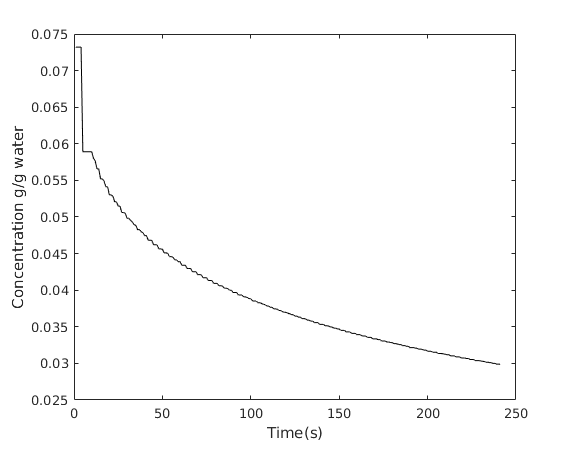
\includegraphics[width=4in]{AppConc.png}
\end{center}
\caption{Concentration Profile}
\end{figure}

The value for the temperature profile was obtained as :
\begin{figure}[h!] 
\begin{center}
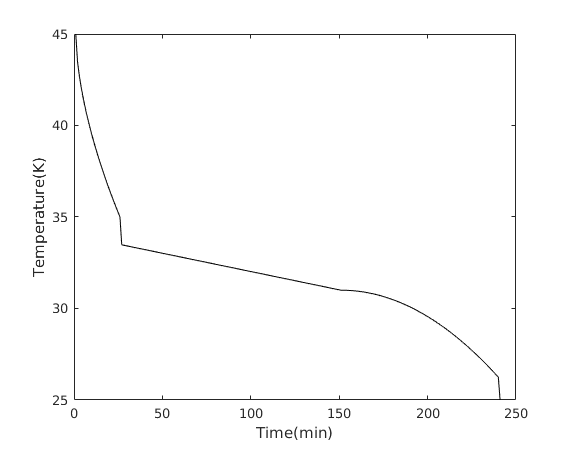
\includegraphics[width=4in]{AppTemp.png}
\end{center}
\caption{Temperature Profile}
\end{figure}

\section{Conclusion}

\begin{itemize}
\item The final value of the objective function($\mu_{4}/\mu_{3}$), ie. the mean crystal size was obtained at : $300 \mu m$
\item The model performs at par with other cooling policies such as cubic cooling policy($251 \mu m$)\cite{bhoi}. This proves the efficacy of P.C.E in the field of batch crystallization.
\end{itemize}
